\newpage\section{Opis zabezpieczanej firmy}
Rozdział zawiera charakterystykę firmy, rodzaj prowadzonej działalności, plan budynku oraz spis sprzętu i pracowników. Jest to stan biura sprzed zabezpieczenia.

\subsection{Charakterystyka firmy}
Firma jest biurem rachunkowym specjalizującym się w doradztwie \linebreak finansowym, prowadzaniu księgowości dla przedsiębiorstw oraz przygotowywaniu analizy finansowej rynku. Przedsiębiorstwo zatrudnia 39 osób, które tworzą cztery działy: dział ekonomistów, dział sprzedaży, dział IT i dział obsługi.

\subsection{Opis budynku}
Dwupiętrowy budynek firmy zlokalizowany jest na obrzeżach dużego miasta. W okolicy jest pomijalnie niskie ryzyko wystąpienia klęsk \linebreak żywiołowych. Budynek otaczają stare drzewa, których nie można wyciąć, ponieważ objęte są ochroną gatunkową. Do przedsiębiorstwa doprowadzona jest sieć telefoniczna oraz internetowa.

Pomieszczenia w budynku zostały zaprojektowane bez uwzględnienia podłogi technicznej, ani sufitu podwieszanego. Urządzania typu routery (Access Point), switche, kamery, alarmy itp. zostały zamontowane na ścianie lub bezpośredniość w suficie. Przewody zasilające oraz sieciowe poprowadzone są w listwach wzdłuż ścian.

Schemat rozmieszczenie pomieszczeń na parterze i piętrze znajduje się odpowiednio na Rys. \ref{schemat:uklad_pomieszczen_poziom0} i \ref{schemat:uklad_pomieszczen_poziom1}.

\begin{landscape}
	\begin{figure}[!h]
		\vspace{3cm}
		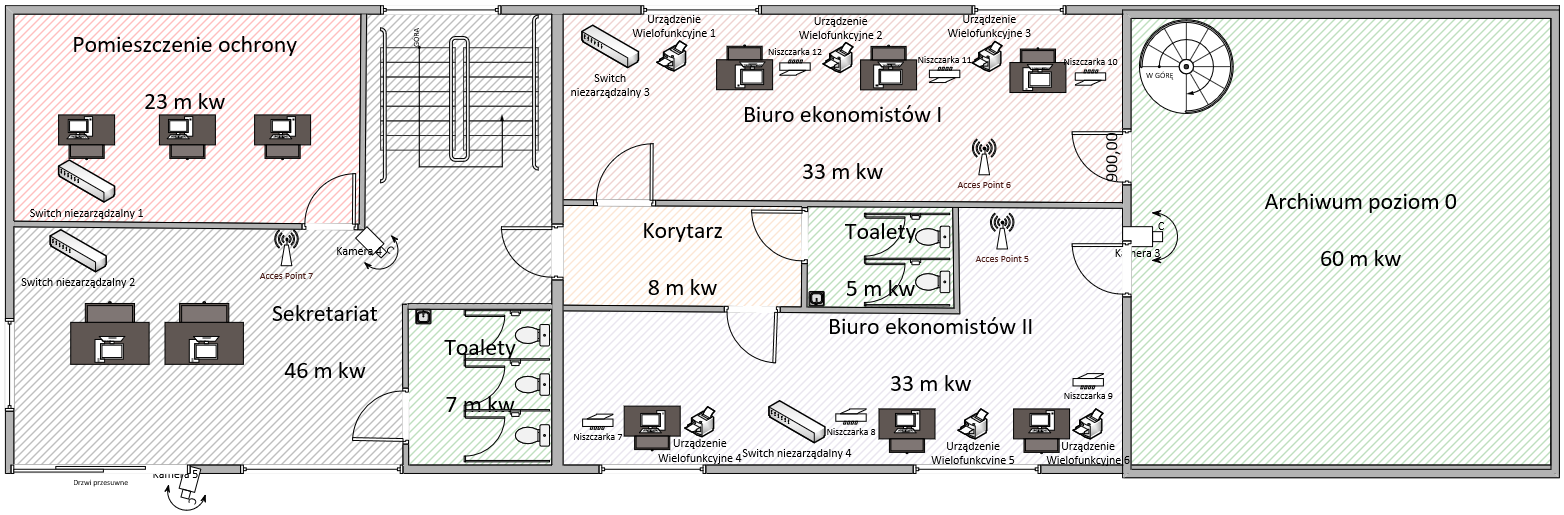
\includegraphics[width=24cm]{uklad_pomieszczen_poziom0.png}
		\caption{Układ pomieszczeń na parterze}
		\label{schemat:uklad_pomieszczen_poziom0}
	\end{figure}
\end{landscape}

\begin{landscape}
	\begin{figure}[!h]
		\vspace{3cm}
		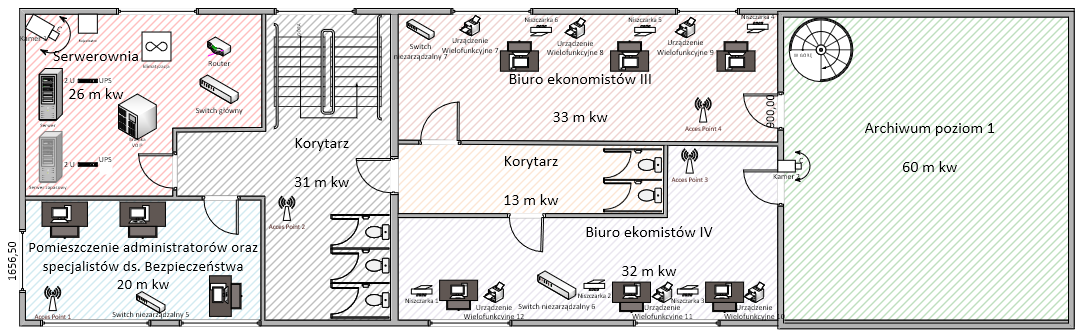
\includegraphics[width=24cm]{uklad_pomieszczen_poziom1.png}
		\caption{Układ pomieszczeń na piętrze}
		\label{schemat:uklad_pomieszczen_poziom1}
	\end{figure}
\end{landscape}

\newpage
\subsection{Sprzęt oraz oprogramowanie}
Poniżej wymieniony został sprzęt informatyczny znajdujący się w firmie wraz z jego podstawowymi parametrami:

\begin{minipage}[\right]{15cm}
\begin{itemize*}
	\item urządzenie wielofunkcyjne Canon PIXMA G3400 (12 sztuk),
	\item niszczarka ProfiOffice PIRANHA EC 7 CC (12 sztuk),
	\item komputer stacjonarny (21 sztuk):
	\begin{itemize*}
		\item procesor Intel i5,
		\item pamięć 8 GB RAM DDR3,
		\item dysk 1 TB HDD,
	\end{itemize*}
	\item laptop DELL Inspiron 5567 (dział IT 6 sztuk),
	\item telefon VoIP Cisco CP-7940G (21 sztuk),
	\item laptop DELL Inspiron 5567 (6 sztuk),
	\item serwer główny (1 sztuka):
	\begin{itemize*}
		\item płyta główna: Intel S2600CP4,
		\item procesor Intel Xeon e5-2603 v2,
		\item pamięć 128 GB RAM DDR3,
		\item dyski SSD o łącznej pojemności 40 TB, 
	\end{itemize*}
	\item serwer zapasowy (1 sztuka):
	\begin{itemize*}
		\item płyta główna: Intel S2600CP4,
		\item procesor Intel Xeon e5-2603 v2,
		\item pamięć 16 GB RAM DDR3,
		\item dyski SSD o łącznej pojemności 10 TB, 
	\end{itemize*}
	\item router Cisco RV325 (1 sztuka),
	\item switch główny Cisco SG300-52 (1 sztuka),
	\item bramka VoIP Grandstream HT704 (1 sztuka),
	\item switch niezarządzalny Cisco SB SF100D-16EU (7 sztuk),
	\item punkt dostępowy Asus RP-AC87 (7 sztuk),
	\item okablowanie:
	\begin{itemize*}
		\item między serwerami 1 Gb/s,
		\item w pozostałych połączeniach skrętka 100 Mb/s,
	\end{itemize*}
	\item UPS VOLT Micro 1200 (1 sztuka),
	\item monitoring:
	\begin{itemize*}
		\item rejestrator BCS-P-QDVR0801ME z dyskiem 2 TB HDD (1 sztuka),
		\item kamera LV-IP2301IP (5 sztuk),
	\end{itemize*}
	\item taśmy magnetyczne.
\end{itemize*}
\end{minipage}

\newpage
Poniżej znajduje się spis oprogramowania (licencji) jakie jest \linebreak zainstalowane w komputerach:

\begin{minipage}[\right]{15cm}
\begin{itemize}
	\item komputery pracowników w dziale ekonomistów:
	\begin{itemize}
		\item Windows 10 (18 sztuk),
		\item pakiet Office 2016 (18 sztuk),
		\item pakiet Insert GT (18 sztuk),
		\item Windows Defender (18 sztuk),
	\end{itemize}
	\item komputery sekretariatu i działu sprzedaży:
	\begin{itemize}
		\item Windows 10 (3 sztuk),
		\item pakiet Office 2016 (3 sztuk),
		\item Windows Defender (3 sztuk),
	\end{itemize}
	\item komputery pracowników w dziale IT:
	\begin{itemize}
		\item Windows 10 (6 sztuk),
		\item pakiet Office 2016 (6 sztuk),
		\item pakiet Insert GT (6 sztuk),
		\item Windows Defender (6 sztuk),
	\end{itemize}
	\item oprogramowanie serwera i wykorzystywane technologie:
	\begin{itemize}
		\item Linux Ubuntu 16.04 LTS z OpenStack (umożliwia wirtualizację
		\linebreak dowolnego systemu),
		\item bazy danych MSSQL,
		\item bazy danych MySQL,
		\item OpenVPN,
		\item Windows Server 2016 (5 sztuk),
		\item Linux Debian 8,
		\item Pakiet Insert GT ( sztuk),
		\item system pocztowy Exim i Dovecot:
		\begin{itemize}
			\item Roundcube jako klient poczty w przeglądarce.
		\end{itemize}
	\end{itemize}
\end{itemize}
\end{minipage}

\newpage
\subsection{Schemat sieci informatycznej}
Sieci informatyczna składa się z routera do którego podłączony jest \linebreak Internet (poprzez światłowód), switcha głównego, 7 switchy niezarządzanych, centrali VoIP oraz 7 punktów dostępowych. Schemat sieci przedstawiony jest na Rys. \ref{schemat:schemat_sieci_infor}. Oznaczenie trzech kropek symbolizuje możliwość podpięcia wielu urządzeń do sieci.

\begin{figure}[!h]
	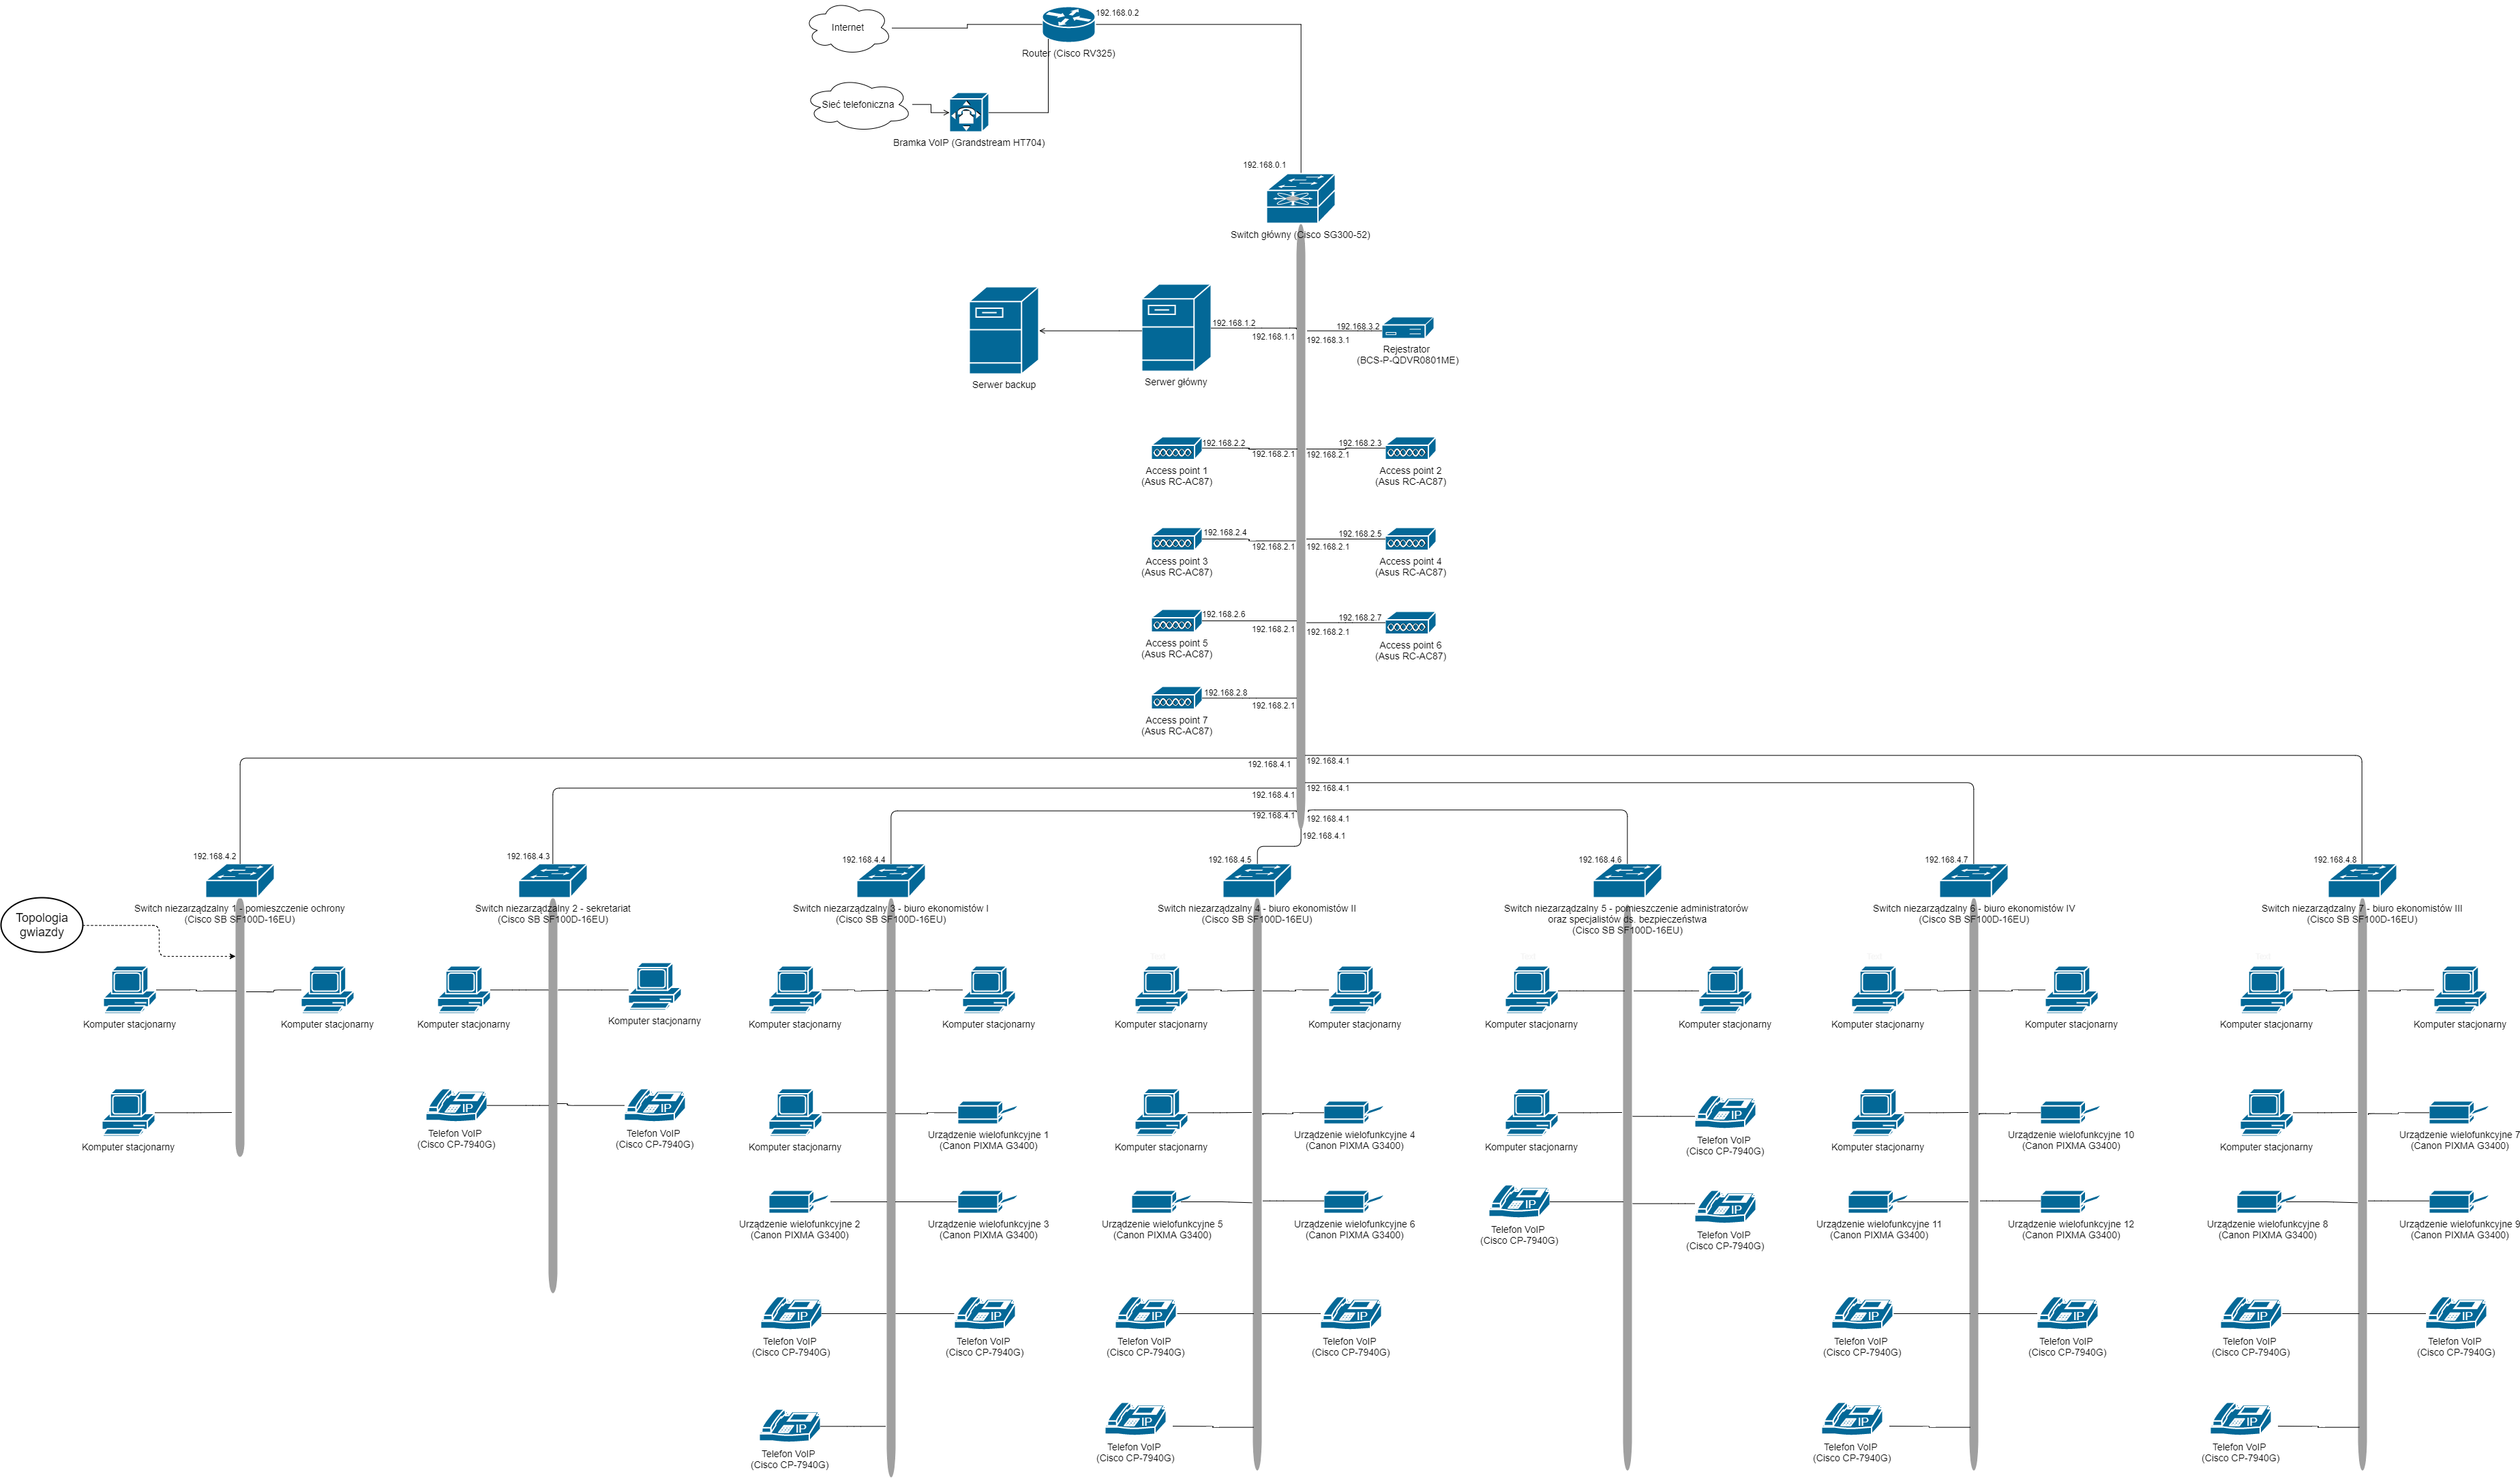
\includegraphics[width=15cm]{Schemat_sieci.png}
	\caption{Schemat sieci informatycznej}
	\label{schemat:schemat_sieci_infor}
\end{figure}

\newpage
Adresacja sieci:

\begin{minipage}[\right]{15cm}
\begin{itemize*}
	\item Router --- brama VoIP --- switch główny:
	\begin{itemize*}
		\item Adres sieci: 192.168.0.0,
		\item Maska sieci: 255.255.255.0,
	\end{itemize*}
	\item Switch główny --- serwer główny:
	\begin{itemize*}
		\item Adres sieci: 192.168.1.0,
		\item Maska sieci: 255.255.255.0,
	\end{itemize*}
	\item Switch główny --- access pointy --- urządzenia podłączone przez WiFi:
	\begin{itemize*}
		\item Adres sieci: 192.168.2.0,
		\item Maska sieci: 255.255.255.0,
	\end{itemize*}
	\item Switch główny --- rejestrator:
	\begin{itemize*}
		\item Adres sieci: 192.168.3.0,
		\item Maska sieci: 255.255.255.0,
	\end{itemize*}
	\item Switch główny --- urządzenia podłączone do switchy niezarządzalnych:
	\begin{itemize*}
		\item Adres sieci: 192.168.4.0,
		\item Maska sieci: 255.255.255.0,
	\end{itemize*}
\end{itemize*}
\end{minipage}

\newpage
\subsection{Organizacja pracy}

\newpage
\subsection{Przechowywane dane}

